% XeLaTeX document
\documentclass[12pt,a4paper]{article}

% Редактируем: конфигурация, личные настройки: имя, название предмета и пр. для титульной страницы и метаданных документа здесь
\newcommand{\university}{Санкт-Петербургский политехнический университет Петра Великого}
\newcommand{\faculty}{Институт компьютерных наук и кибербезопасности}
\newcommand{\department}{Высшая школа компьютерных технологий и информационных систем}
\newcommand{\city}{Санкт-Петербург}
\newcommand{\num}{ №12}
\newcommand{\docname}{Лабораторная работа}
\newcommand{\subject}{Телекоммуникационные технологии}
\newcommand{\tutorname}{Богач Н. В.}
\newcommand{\studentname}{Граур А. А.}
\newcommand{\group}{5130901/10203}

% Не редактируем: используемые пакеты
% настройка кодировки, шрифтов и русского языка
\usepackage{fontspec}
\usepackage{polyglossia}

% рабочие ссылки в документе
\usepackage{hyperref}

% графика
\usepackage{graphicx}
\usepackage{tikz}

% поворот страницы
\usepackage{pdflscape}

% качественные листинги кода
\usepackage{minted}
\usepackage{listings}
\usepackage{lstfiracode}

% отключение копирования номеров строк из листинга, работает не во всех просмотрщиках (в Adobe Reader работает)
\usepackage{accsupp}
\newcommand\emptyaccsupp[1]{\BeginAccSupp{ActualText={}}#1\EndAccSupp{}}
\let\theHFancyVerbLine\theFancyVerbLine
\def\theFancyVerbLine{\rmfamily\tiny\emptyaccsupp{\arabic{FancyVerbLine}}}

\usepackage{csquotes}

% установка полей
\usepackage{geometry}

% нумерация картинок по секциям
\usepackage{chngcntr}

% дополнительные команды для таблиц
\usepackage{booktabs}

% для заголовков
\usepackage{caption}
\usepackage{titlesec}
\usepackage[dotinlabels]{titletoc}

% разное для математики
\usepackage{amsmath, amsfonts, amssymb, amsthm, mathtools}

% водяной знак на документе, см. main.tex
\usepackage[printwatermark]{xwatermark}

% Не редактируем: параметры используемых пакетов и не только
% настройки polyglossia
\setdefaultlanguage{russian}
\setotherlanguage{english}

% локализация
\addto\captionsrussian{
	\renewcommand{\figurename}{Figure}%
	\renewcommand{\partname}{Part}
	\renewcommand{\contentsname}{\centerline{Содержание}}
	\renewcommand{\listingscaption}{Listing}
}

% основной шрифт документа
\setmainfont{CMU Serif}
\newfontfamily\cyrillicfont{CMU Serif}[Script=Cyrillic]

% настройка полей
\geometry{top=2cm}
\geometry{bottom=2cm}
\geometry{left=2cm}
\geometry{right=2cm}
\geometry{bindingoffset=0cm}

% настройка ссылок и метаданных документа
\hypersetup{unicode=true,colorlinks=true,linkcolor=red,citecolor=green,filecolor=magenta,urlcolor=cyan,
	pdftitle={\docname},
	pdfauthor={\studentname},
	pdfsubject={\subject},
	pdfcreator={\studentname},
	pdfproducer={Overleaf},
	pdfkeywords={\subject}
}

% настройка подсветки кода и окружения для листингов
\usemintedstyle{colorful}
\newenvironment{code}{\captionsetup{type=listing}}{}

% шрифт для листингов с лигатурами
\setmonofont{FiraCode-Regular.otf}[
	SizeFeatures={Size=10},
	Path = templates/,
	Contextuals=Alternate
]

% оформления подписи рисунка
\captionsetup[figure]{labelsep = period}

% подпись таблицы
\DeclareCaptionFormat{hfillstart}{\hfill#1#2#3\par}
\captionsetup[table]{format=hfillstart,labelsep=newline,justification=centering,skip=-10pt,textfont=bf}

% путь к каталогу с рисунками
\graphicspath{{fig/}}

% Внесение titlepage в учёт счётчика страниц
\makeatletter
\renewenvironment{titlepage} {
	\thispagestyle{empty}
}
\makeatother

\counterwithin{figure}{section}
\counterwithin{table}{section}

\titlelabel{\thetitle.\quad}

% для удобного конспектирования математики
\mathtoolsset{showonlyrefs=true}
\theoremstyle{plain}
\newtheorem{theorem}{Теорема}[section]
\newtheorem{proposition}[theorem]{Утверждение}
\theoremstyle{definition}
\newtheorem{corollary}{Следствие}[theorem]
\newtheorem{problem}{Задача}[section]
\theoremstyle{remark}
\newtheorem*{nonum}{Решение}

% настоящее матожидание
\newcommand{\MExpect}{\mathsf{M}}

% объявили оператор!
\DeclareMathOperator{\sgn}{\mathop{sgn}}

% перенос знаков в формулах (по Львовскому)
\newcommand*{\hm}[1]{#1\nobreak\discretionary{} {\hbox{$\mathsurround=0pt #1$}}{}}


% водяной знак для обозначения статуса документа
% \newwatermark[allpages,color=red!5,angle=45,scale=3,xpos=0,ypos=0]{DRAFT}
\begin{document}
% Не редактируем: Титульная страница (формируется автоматически из заданной конфигурации)
\begin{titlepage}	% начало титульной страницы

	\begin{center}		% выравнивание по центру

		\large \university \\
		\large \faculty \\
		\large \department \\[6cm]
		% название института, затем отступ 6см

		\huge \subject \\[0.5cm] % название работы, затем отступ 0,5см
		\large \docname \num \\[5.1cm]
		% \large Тема работы\\[5cm]

	\end{center}


	\begin{flushright} % выравнивание по правому краю
		\begin{minipage}{0.25\textwidth} % врезка в половину ширины текста
			\begin{flushleft} % выровнять её содержимое по левому краю

				\large\textbf{Работу выполнил:}\\
				\large \studentname \\
				\large {Группа:} \group \\

				\large \textbf{Преподаватель:}\\
				\large \tutorname

			\end{flushleft}
		\end{minipage}
	\end{flushright}

	\vfill % заполнить всё доступное ниже пространство

	\begin{center}
		\large \city \\
		\large \the\year % вывести дату
	\end{center} % закончить выравнивание по центру

\end{titlepage} % конец титульной страницы

\vfill % заполнить всё доступное ниже пространство


% Не редактируем: Страница содержания (формируется автоматически из section, subsection и пр., указанных в content.tex)
% Содержание
\tableofcontents
\newpage



% Редактируем: всё остальное: вступление, др. этапы, заключение, приложение
\section{Designing Filter Taps}

Демонстрирует, как создать список или массив коэффициентов фильтра и применить их в блоке низкочастотной фильтрации.

\subsection{Проектирование коэффициентов фильтра}

Начнем с блок-схемы из примера низкочастотного фильтра, но заменим низкочастотный фильтр на частотно-смещенный FIR фильтр и добавим блок Low-Pass Filter Taps:

\begin{center}
    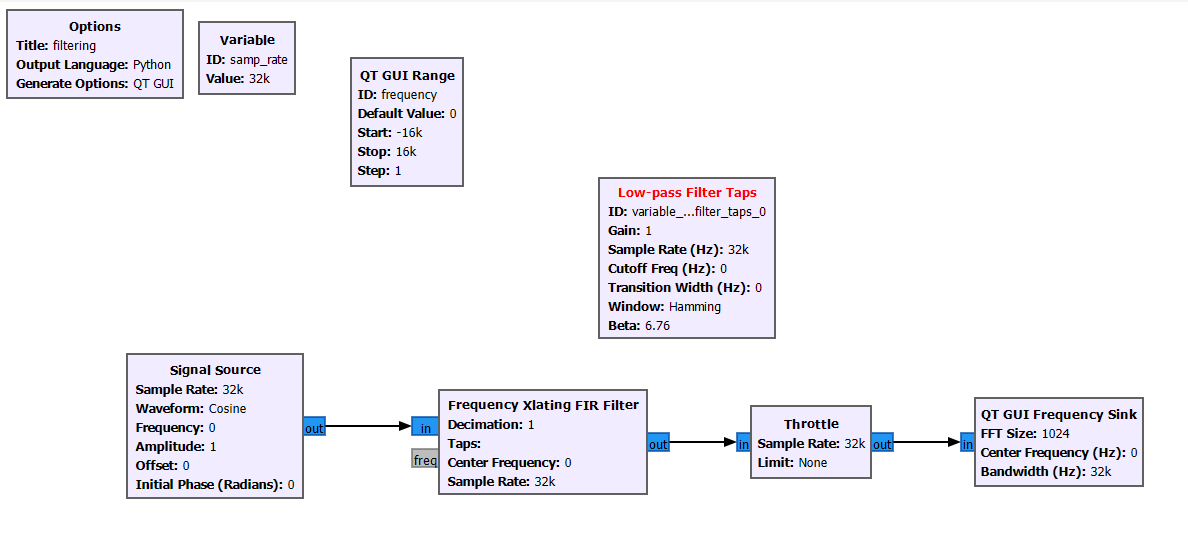
\includegraphics[width=0.8\textwidth]{1}
\end{center}

Блок Low-Pass Filter Taps задает набор коэффициентов фильтра, которые можно применять к блокам фильтрации. Коэффициенты фильтра также могут называться весами или коэффициентами. Ответ и производительность фильтра зависят от параметров, введенных пользователем. Дважды щелкнем по блоку Low-Pass Filter Taps, чтобы открыть свойства. Отредактируем их:

\begin{itemize}
    \item Id: \verb|lowPassFilterTaps|
    \item Cutoff Freq (Hz): \verb|samp_rate/4|
    \item Transition Width (Hz): \verb|samp_rate/8|
\end{itemize}

\begin{center}
    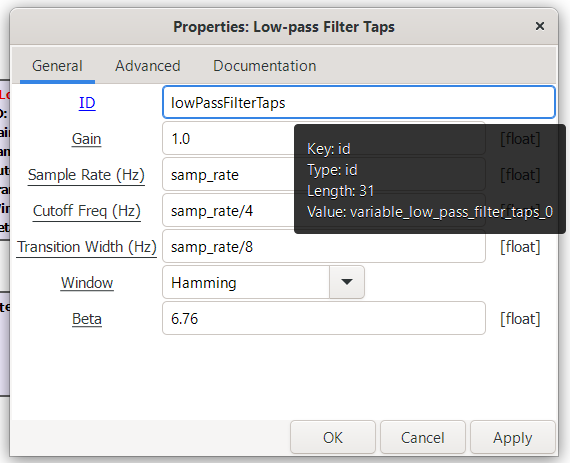
\includegraphics[width=0.5\textwidth]{2}
\end{center}

Блок Low-Pass Filter Taps сохраняет коэффициенты фильтра в список в переменной lowPassFilterTaps.

Дважды щелкнем по блоку частотно-смещенного FIR фильтра, чтобы отредактировать свойства. Введем \verb|lowPassFilterTaps| для параметра Taps. Наведение курсора на переменную lowPassFilterTaps отображает информацию о коэффициентах фильтра:

\begin{center}
    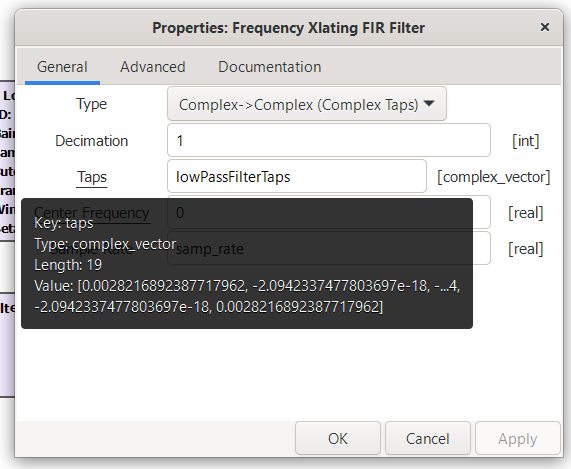
\includegraphics[width=0.8\textwidth]{3}
\end{center}

Первые несколько коэффициентов фильтра отображаются в списке. Сохраним свойства и запустим flowgraph:

\begin{center}
    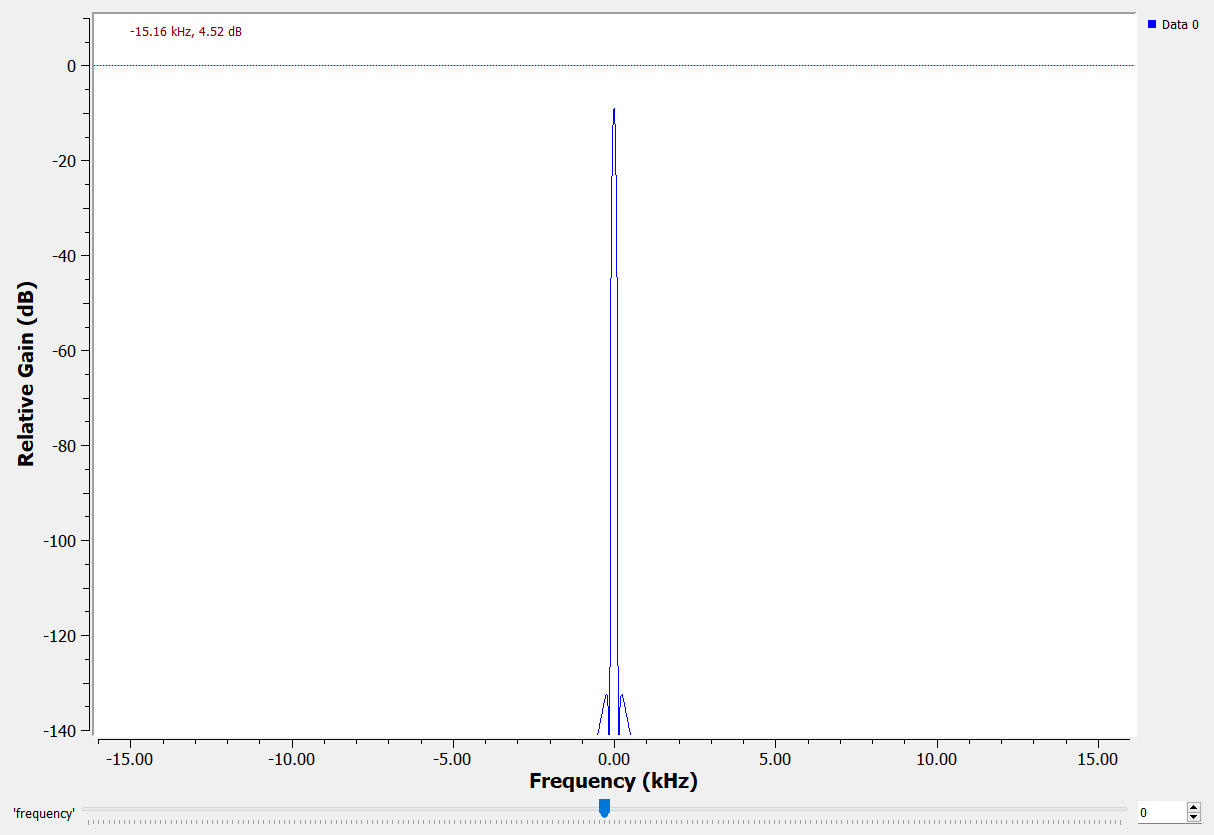
\includegraphics[width=0.8\textwidth]{4}
\end{center}

Попробуем поизменять частоту. Амплитуда частотной характеристики затем может быть видна через контур:

\begin{center}
    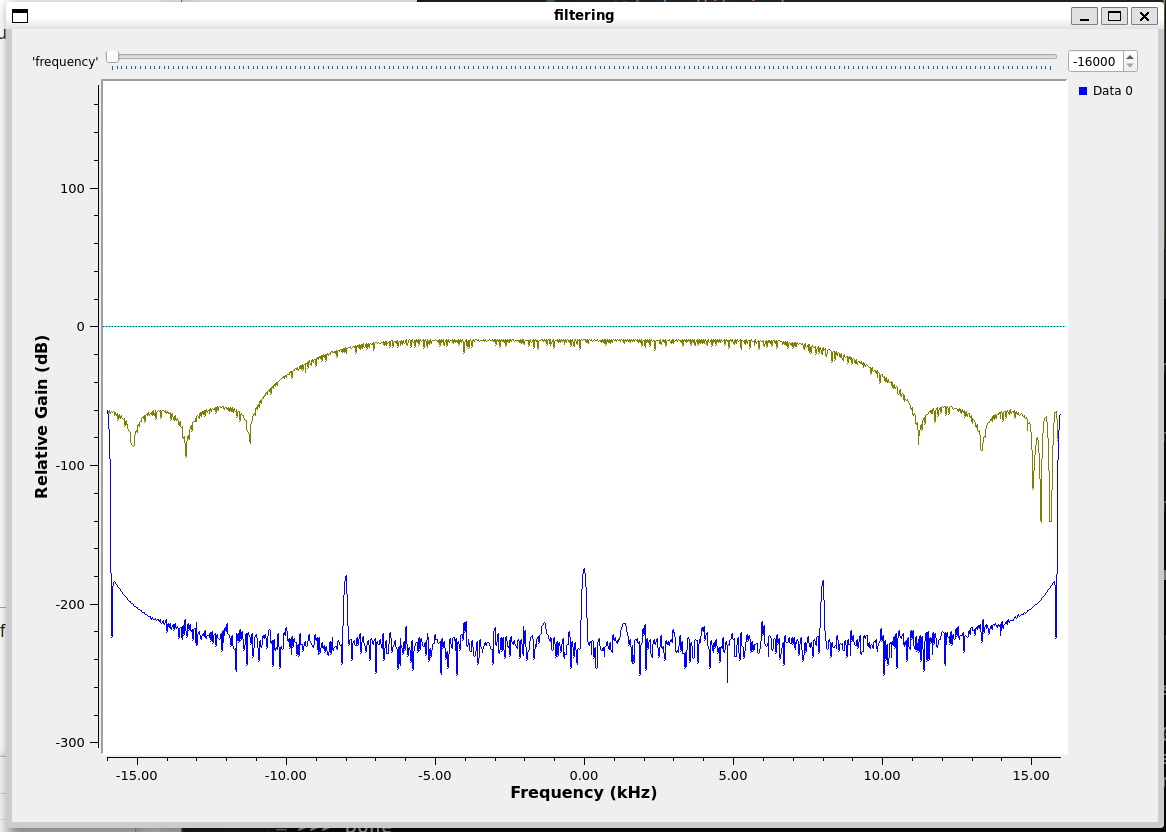
\includegraphics[width=0.8\textwidth]{5}
\end{center}

\subsection{Ввод коэффициентов фильтра вручную}

Альтернативные методы могут использоваться для задания коэффициентов фильтра, а затем ввода их вручную в виде переменной в Python. Например, блок частотно-смещенного FIR фильтра принимает коэффициенты фильтра в виде массива NumPy. Добавим блок Import в рабочее пространство GRC:

\begin{center}
    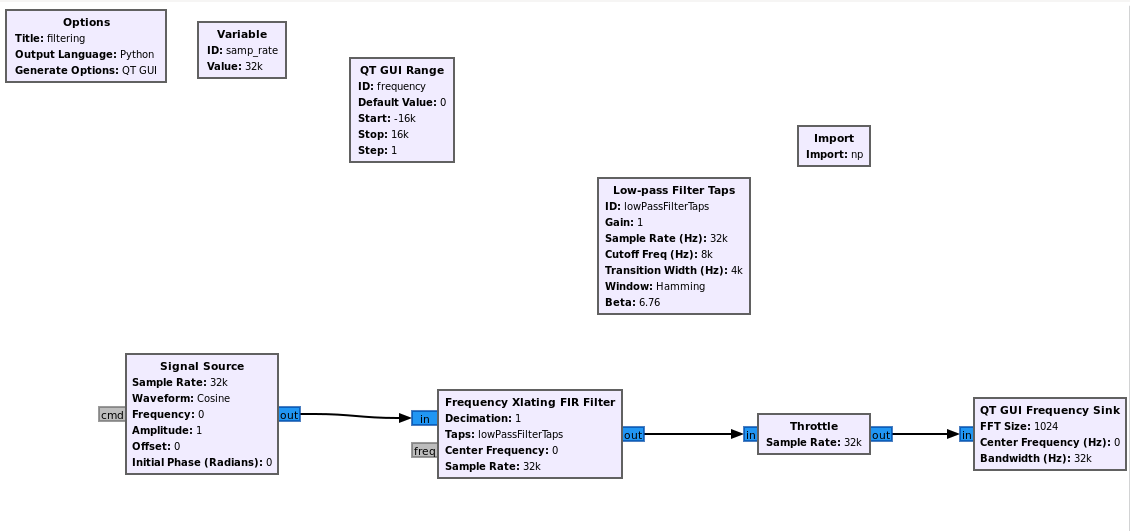
\includegraphics[width=0.8\textwidth]{6}
\end{center}

\begin{center}
    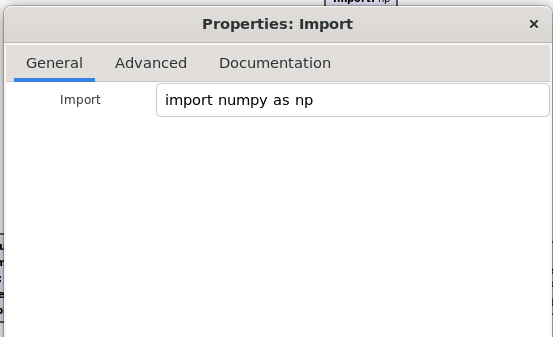
\includegraphics[width=0.8\textwidth]{7}
\end{center}

Простой фильтр скользящего среднего или \verb|boxcar| можно задать, установив все коэффициенты фильтра одинаковыми. Это можно сделать с помощью функции NumPy ones(), которая возвращает массив NumPy, состоящий из единиц указанной длины. Создадим переменную с именем boxcarFilter со значением:

\begin{verbatim}
boxcarFilter = np.ones(10)
\end{verbatim}

\begin{center}
    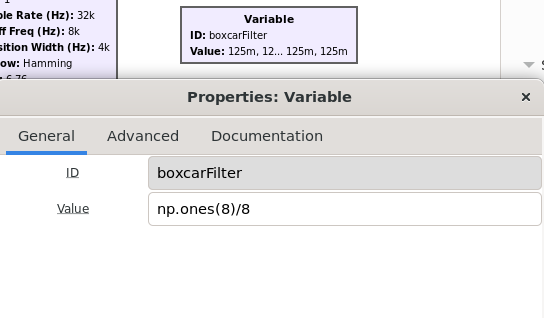
\includegraphics[width=0.8\textwidth]{8}
\end{center}

Отключим Low-Pass Filter Taps и заменим его на \verb|boxcarFilter| в Frequency Xlating FIR Filter. Блок-схема выглядит следующим образом:

\begin{center}
    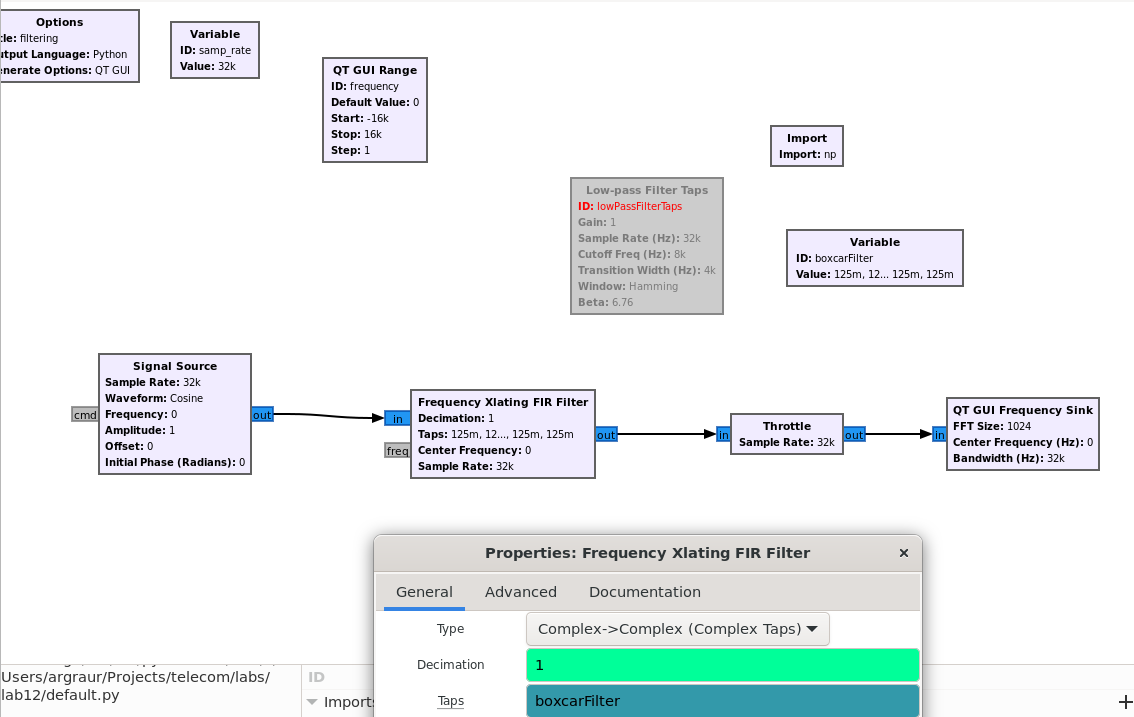
\includegraphics[width=0.8\textwidth]{9}
\end{center}

Теперь можно увидеть другую амплитуду частотной характеристики, поскольку используются разные коэффициенты фильтра:

\begin{center}
    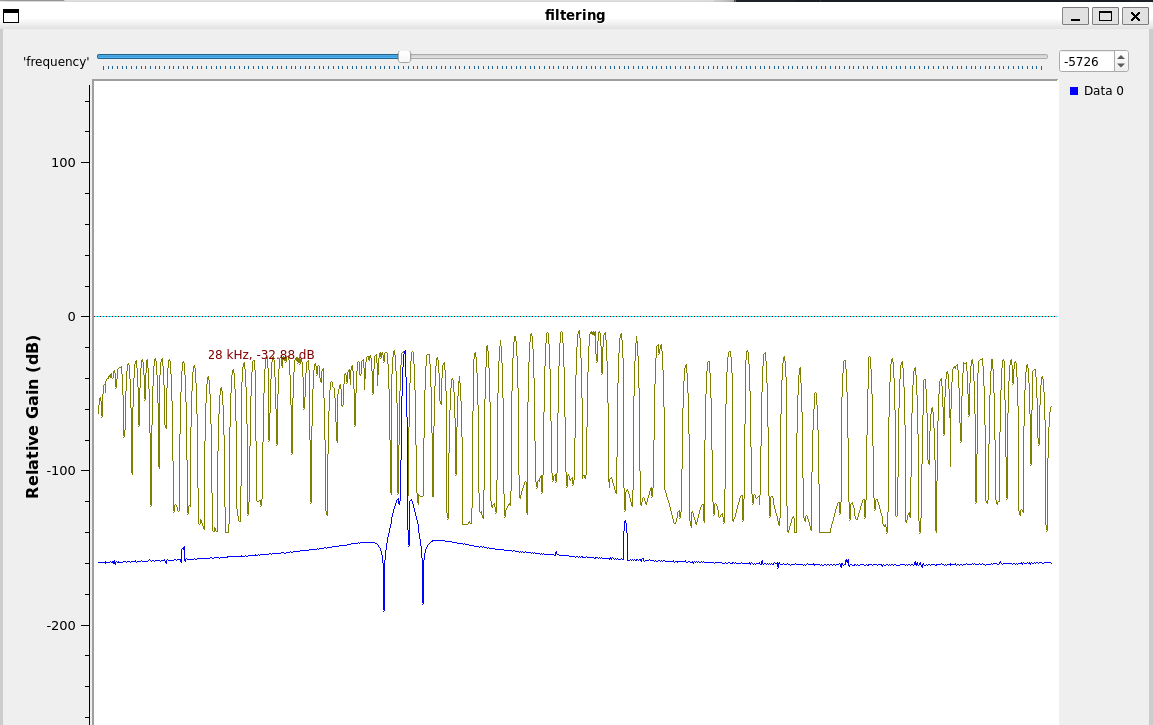
\includegraphics[width=0.8\textwidth]{10}
\end{center}

\subsection{Фильтр от реального к комплексному}

Многие блоки фильтрации имеют опции выбора комбинаций реальных или комплексных типов данных для входа и выхода, а также реальных или комплексных весов фильтра. Этот пример демонстрирует один из методов использования комплексных весов фильтра для преобразования реального сигнала в комплексный. Удалим переменную \verb|boxcarFilter| и снова включим блок Low-Pass Filter Taps:

\begin{center}
    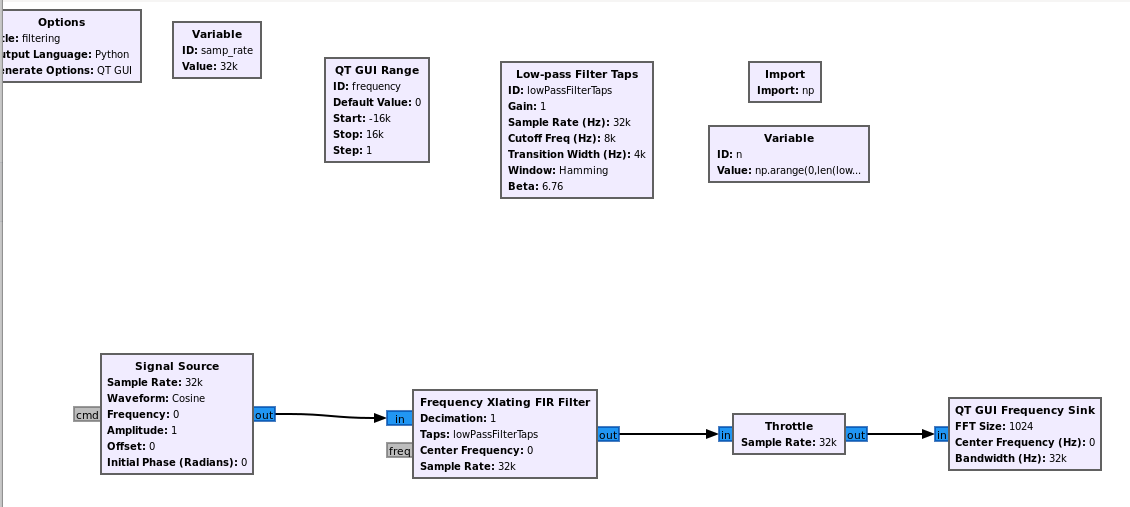
\includegraphics[width=0.8\textwidth]{11}
\end{center}

\verb|lowPassFilterTaps| используются как основа для комплексного полосового фильтра. Создадим переменную \verb|n| со значением:

\begin{verbatim}
np.arange(0,len(lowPassFilterTaps))
\end{verbatim}

которая образует массив целых чисел: 0, 1, 2, 3, ... до длины \verb|lowPassFilterTaps|:

\begin{center}
    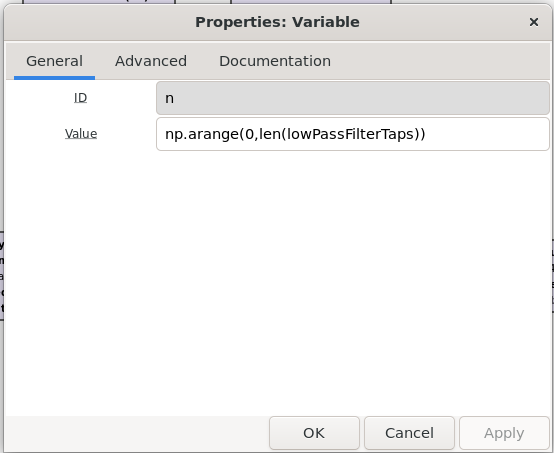
\includegraphics[width=0.8\textwidth]{12}
\end{center}

Создадим переменную \verb|frequencyShift| со значением:

\begin{verbatim}
np.exp(1j * 2 * np.pi * 0.25 * n)
\end{verbatim}

\begin{center}
    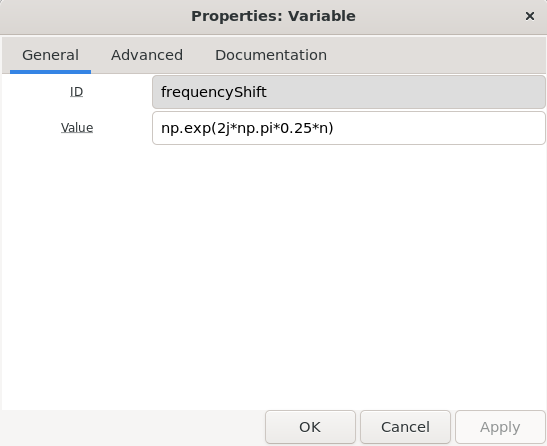
\includegraphics[width=0.8\textwidth]{13}
\end{center}

Эта функция является комплексной синусоидой с частотой \(1/4\) частоты дискретизации. Переменная \verb|frequencyShift| изменяет центральную частоту \verb|lowPassFilterTaps| с \(0\) до \(1/4\) частоты дискретизации. Создадим переменную \verb|bandPassTaps| со значением:

\begin{verbatim}
lowPassFilterTaps * frequencyShift
\end{verbatim}

\begin{center}
    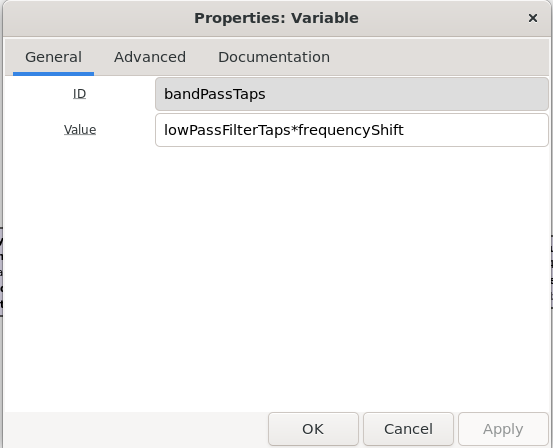
\includegraphics[width=0.8\textwidth]{14}
\end{center}

Отредактируем блок Frequency Xlating FIR Filter. В качестве типа выберем Float->Complex(Complex Taps):

\begin{center}
    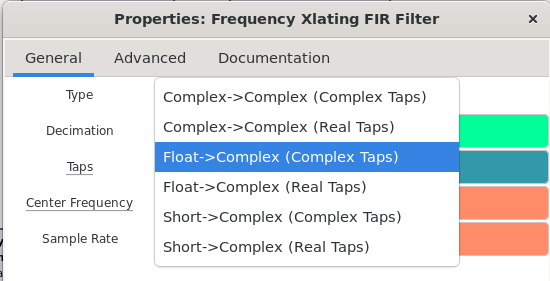
\includegraphics[width=0.8\textwidth]{15}
\end{center}

Заменим lowPassFilterTaps на bandPassTaps в частотно-смещенном фильтре.

Отредактируем свойства источника сигнала и преобразуем его в реальный сигнал.

\begin{center}
    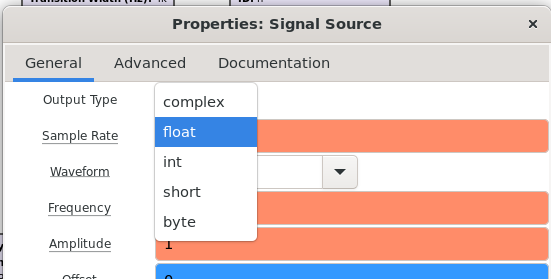
\includegraphics[width=0.8\textwidth]{16}
\end{center}

Блок-схема выглядит следующим образом:

\begin{center}
    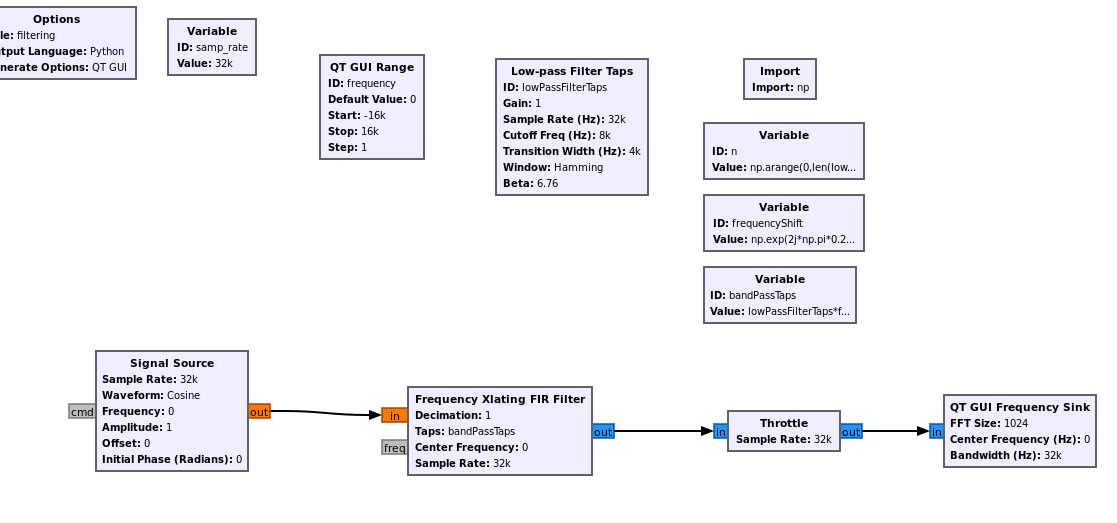
\includegraphics[width=0.8\textwidth]{17}
\end{center}

Запустим блок-схему.

\begin{center}
    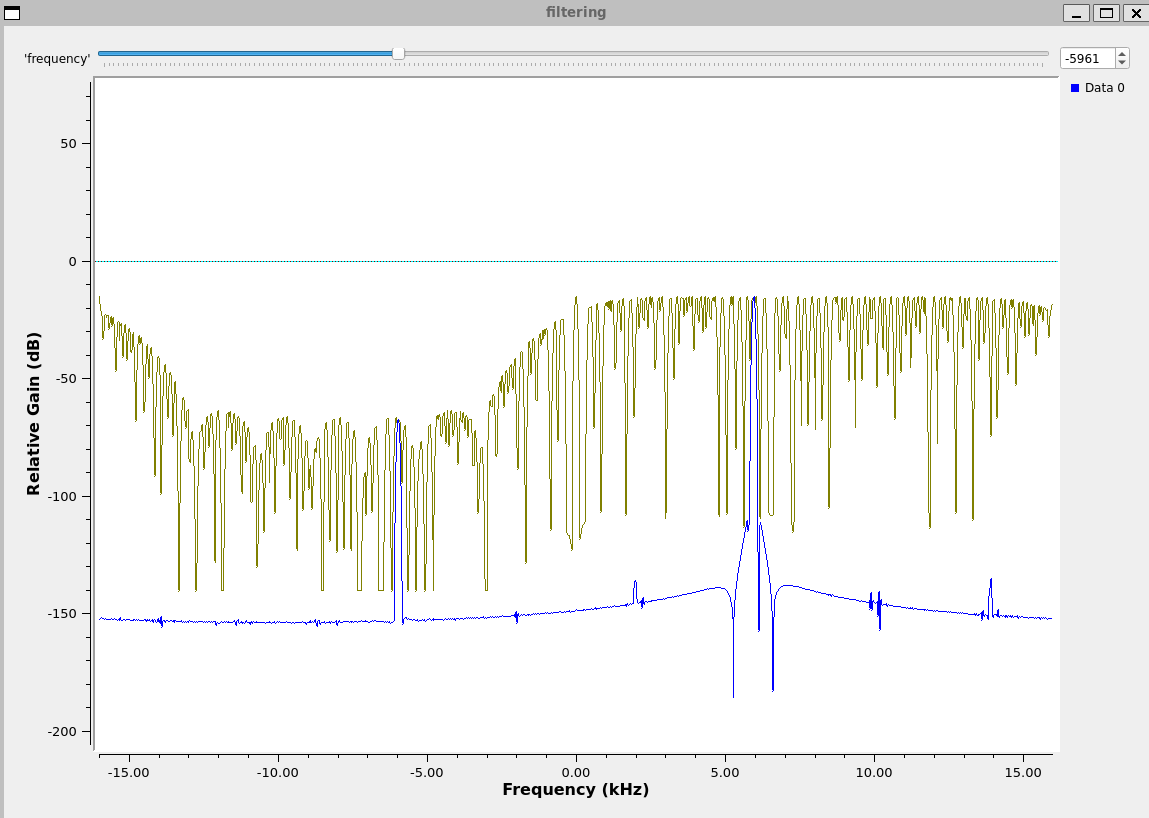
\includegraphics[width=0.8\textwidth]{18}
\end{center}

Амплитуда частотной характеристики показывает, что центральная частота низкочастотного фильтра была смещена до 1/4 частоты дискретизации, что теперь является полосовым фильтром. Частотная характеристика теперь отличается между положительными и отрицательными частотами, что может быть свойством комплексных фильтров (но не реальных фильтров).

\end{document}